\begin{acquis}
\begin{itemize}
\item BlaBla1
\item BlaBla2
\item BlaBla3
\item BlaBla4
\item BlaBla5
\item BlaBla6
\end{itemize}
\end{acquis}

\QCMautoevaluation{Pour chaque question, plusieurs réponses sont
  proposées.  Déterminer celles qui sont correctes.} 
  
\begin{QCM}
  \begin{GroupeQCM} 
    \begin{exercice}
      Si $CA = CB$ alors \ldots
      \begin{ChoixQCM}{4}
      \item $C$ est le milieu de $[AB]$
      \item le triangle $ABC$ est isocèle en $A$
      \item $A$ et $B$ sont sur un cercle de centre $C$
      \item le triangle $ABC$ est isocèle en $C$
      \end{ChoixQCM}
\begin{corrige}
     \reponseQCM{cd} 
   \end{corrige}
    \end{exercice}
    

    \begin{exercice}
      Un triangle $ABC$ est isocèle en $B$ alors \ldots
      \begin{ChoixQCM}{4}
      \item $AC = BC$
      \item $AB = BC$
      \item Le plus grand angle est $\widehat{ABC}$
      \item $\widehat{CAB} = \widehat{BCA}$
      \end{ChoixQCM}
\begin{corrige}
     \reponseQCM{bd}
   \end{corrige}
    \end{exercice}


    \begin{exercice}
      Si $RST$ est un triangle rectangle en $T$ alors \ldots
      \begin{ChoixQCM}{4}
      \item $RS = ST$
      \item $(ST) \perp (RS)$
      \item $(ST) \perp (TR)$
      \item $RS \geqslant ST$ et $RS \geqslant RT$
      \end{ChoixQCM}
\begin{corrige}
     \reponseQCM{cd}
   \end{corrige}
    \end{exercice}
    

    \begin{exercice}
      Sur la figure ci‑dessous, \ldots
      
     \begin{minipage}[c]{0.32\textwidth}
     \quad 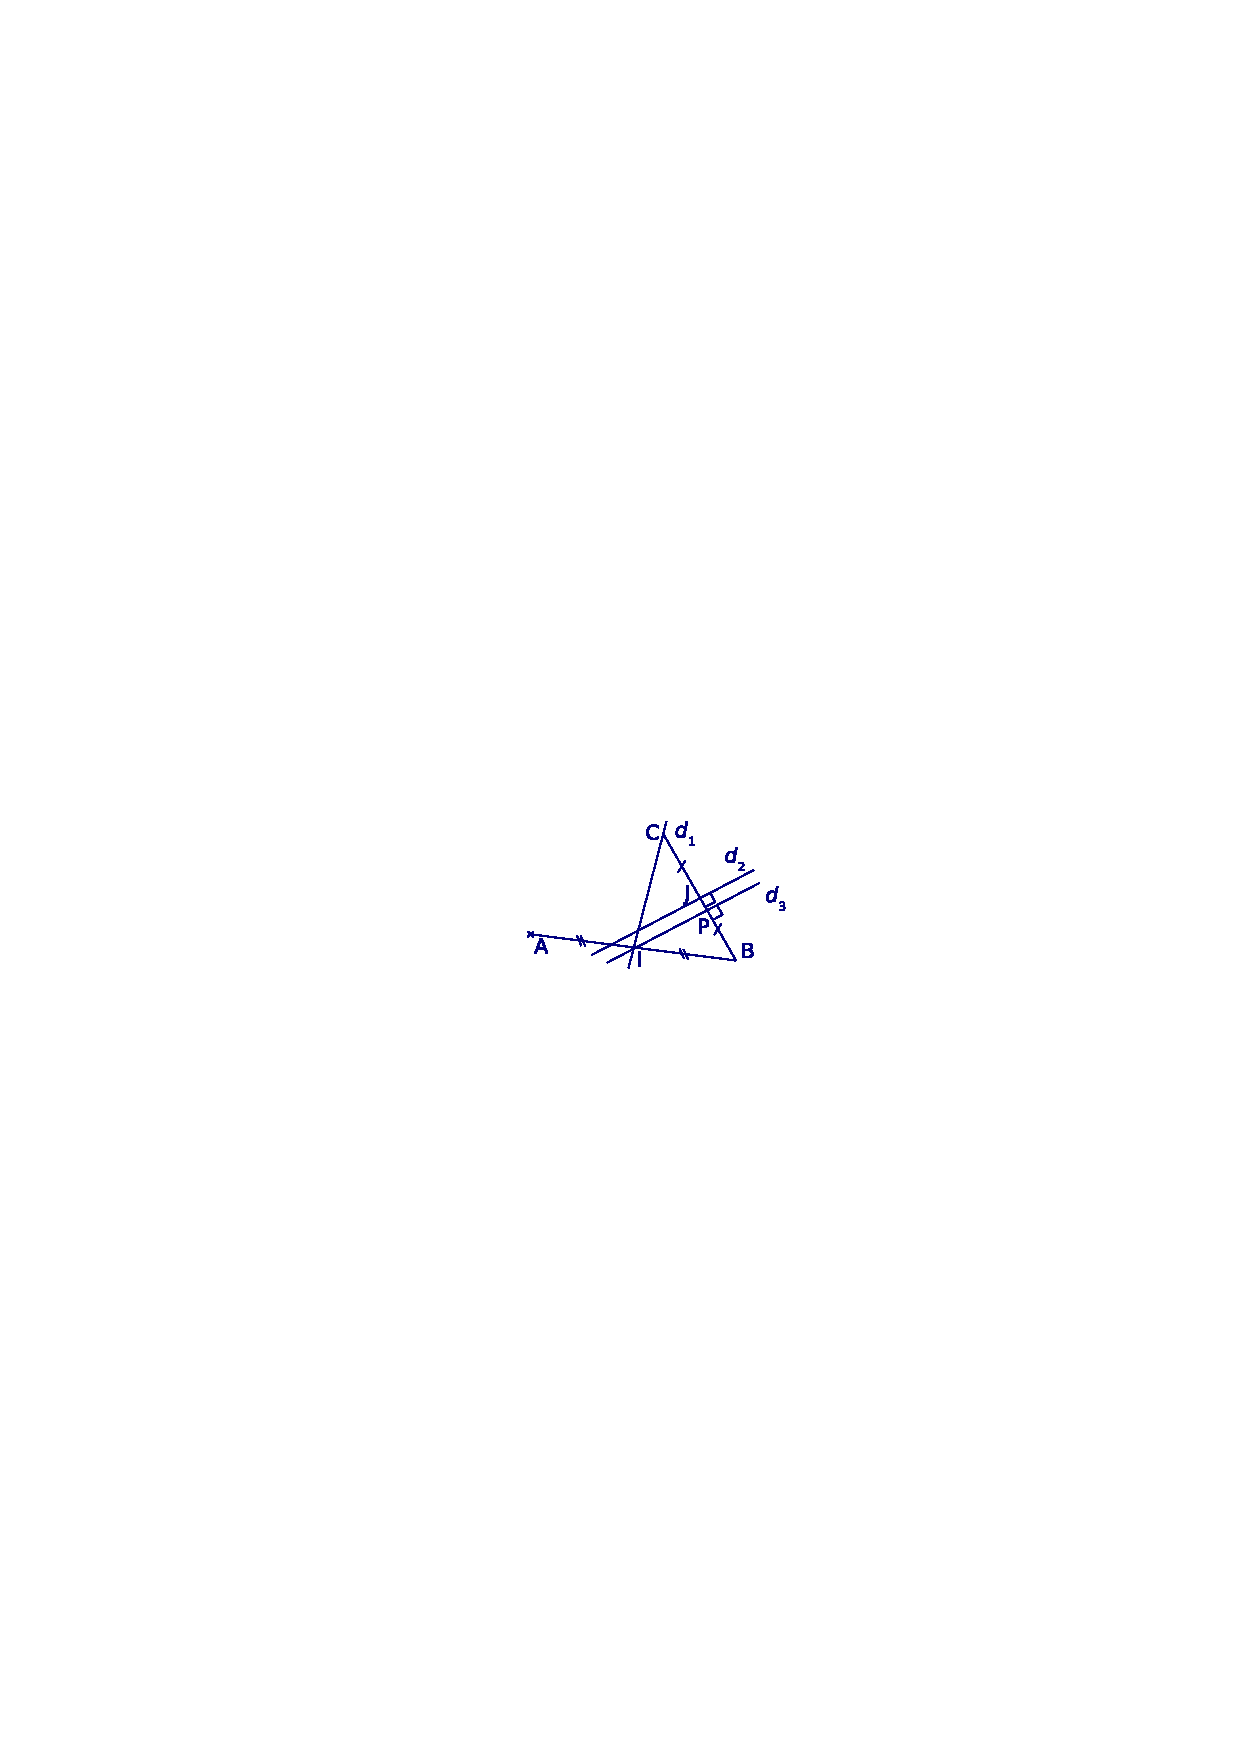
\includegraphics[width=3.5cm]{triangleACIB}
     \end{minipage} \hfill%
     \begin{minipage}[c]{0.66\textwidth}
     $d_1$ correspond à la droite $(CI)$
     
     $AI = IB$ et $CJ = BJ$
     \end{minipage} \\
      
      \begin{ChoixQCM}{4}
      \item la droite $d_1$ est la médiatrice du segment $[AB]$
      \item la droite $d_2$ est la médiatrice du segment $[CB]$
      \item le triangle $BCI$ est un triangle rectangle
      \item $d_3 \parallel (CB)$
      \end{ChoixQCM}
\begin{corrige}
     \reponseQCM{b}
   \end{corrige}
    \end{exercice}
    

\end{GroupeQCM}
\end{QCM}

  